\pagenumbering{roman}
\section{Appendix}
\subsection{Our revised grammar}\label{sec:grammar_revised}

\begin{tabbing}
    $\langle \text{Crn} \rangle$ \,::=\; \= \texttt{'crn=\{'$\langle \text{ConcRootSList} \rangle$'\}'} \\
    
    $\langle \text{ConcRootSList} \rangle$ \,::=\;  $\langle \text{ConcS} \rangle$ ',' $\langle \text{ConcRootList} \rangle$ \\
    \>\textbar \, $\langle \text{RootSList} \rangle$ \\

    $\langle \text{RootSList} \rangle$ \,::=\;  $\langle \text{StepS} \rangle$ \\
    \>\textbar \, $\langle \text{StepS} \rangle$ ',' $\langle \text{RootSList} \rangle$ \\
     
    $\langle \text{ConcS} \rangle$ \,::=\;  \texttt{'conc['$\langle \text{species} \rangle$','$\langle \text{number} \rangle$']'} \\
    
    $\langle \text{StepS} \rangle$ \,::=\;  \texttt{'step['$\langle \text{CommandSList} \rangle$']'} \\
    
    $\langle \text{CommandSList} \rangle$ \,::=\;  $\langle \text{CommandS} \rangle$ \\
    \>\textbar \, $\langle \text{CommandS} \rangle$ \texttt{','} $\langle \text{CommandSList} \rangle$ \\
     
    $\langle \text{CommandS} \rangle$ \,::=\;  \texttt{'rxn['$\langle \text{Expr} \rangle$', '$\langle \text{Expr} \rangle$', '$\langle \text{number} \rangle$']'} \\
    \>\textbar \, \texttt{'ld['$\langle \text{species} \rangle$', '$\langle \text{species} \rangle$']'} \\
    \>\textbar \, \texttt{'add['$\langle \text{species} \rangle$', '$\langle \text{species} \rangle$', '$\langle \text{species} \rangle$']'} \\
    \>\textbar \, \texttt{'sub['$\langle \text{species} \rangle$', '$\langle \text{species} \rangle$', '$\langle \text{species} \rangle$']'} \\
    \>\textbar \, \texttt{'mul['$\langle \text{species} \rangle$', '$\langle \text{species} \rangle$', '$\langle \text{species} \rangle$']'} \\
    \>\textbar \, \texttt{'div['$\langle \text{species} \rangle$', '$\langle \text{species} \rangle$', '$\langle \text{species} \rangle$']'} \\
    \>\textbar \, \texttt{'sqrt['$\langle \text{species} \rangle$', '$\langle \text{species} \rangle$']'} \\
    \>\textbar \, \texttt{'cmp['$\langle \text{species} \rangle$', '$\langle \text{species} \rangle$']'} \\
    \>\textbar \, \texttt{'ifGT['$\langle \text{CommandSList} \rangle$']'} \\
    \>\textbar \, \texttt{'ifGE['$\langle \text{CommandSList} \rangle$']'} \\
    \>\textbar \, \texttt{'ifEQ['$\langle \text{CommandSList} \rangle$']'} \\
    \>\textbar \, \texttt{'ifLT['$\langle \text{CommandSList} \rangle$']'} \\
    \>\textbar \, \texttt{'ifLE['$\langle \text{CommandSList} \rangle$']'} \\
     
    $\langle \text{Expr} \rangle$ \,::=\;  \texttt{$\langle \text{species} \rangle$} \, \{\texttt{'$+$' $\langle \text{species} \rangle$}\}
\end{tabbing}


\subsection{Interpreter plots}\label{sec:interpreter_plots}

\begin{figure}[H]
    \centering
    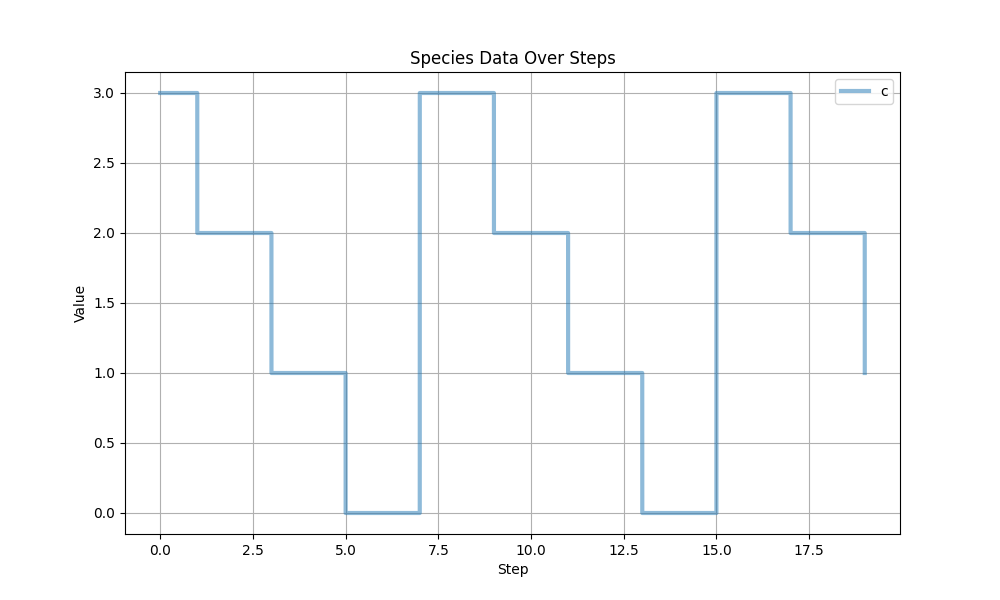
\includegraphics[width=\textwidth]{report/figures/InterpreterPlots/counterInt.png}
    \caption{Discrete counter}
\end{figure}

\begin{figure}[H]
    \centering
    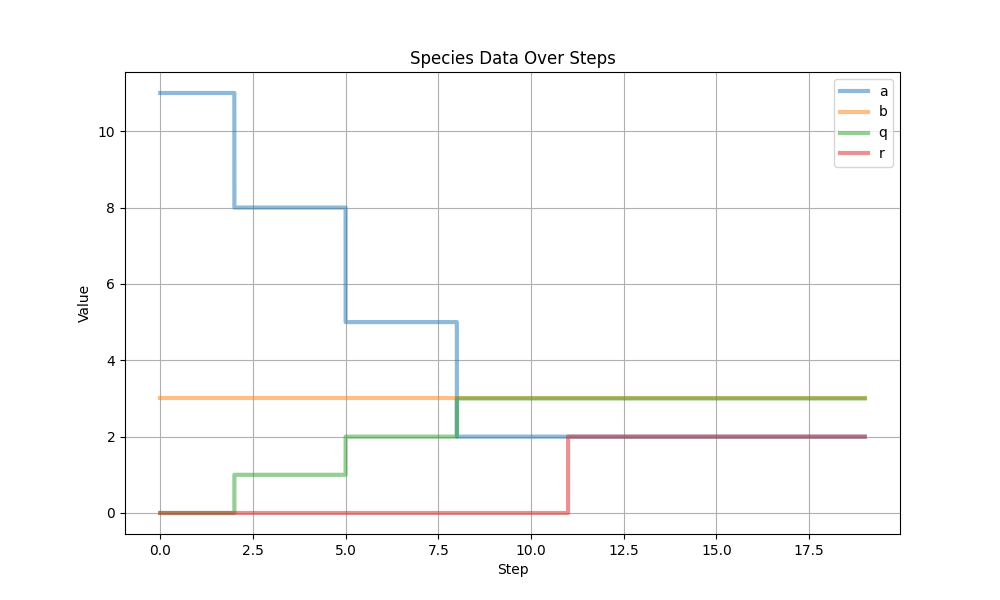
\includegraphics[width=\textwidth]{report/figures/InterpreterPlots/divisionInt.png}
    \caption{Division}
\end{figure}

\begin{figure}[H]
    \centering
    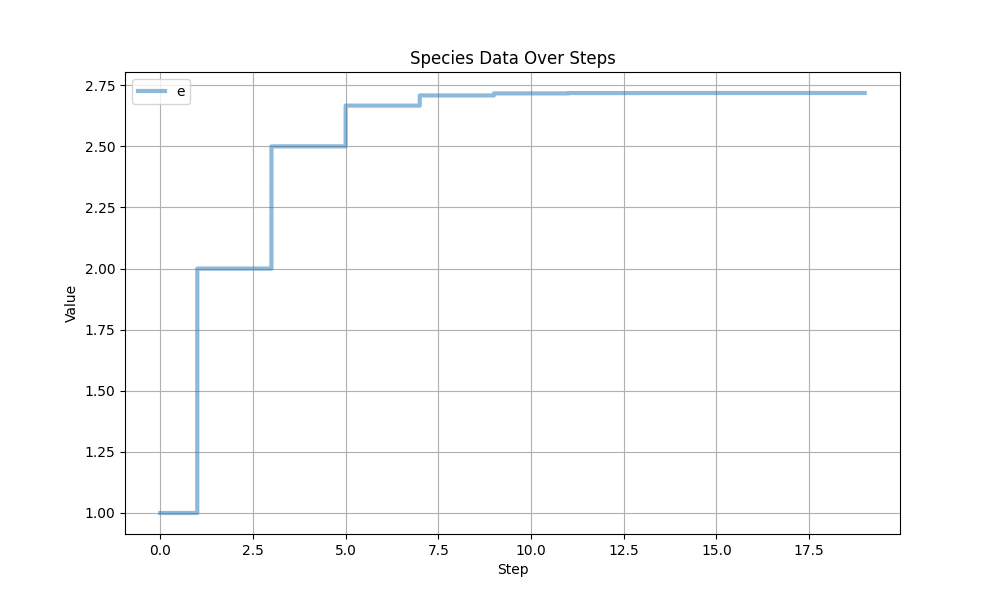
\includegraphics[width=\textwidth]{report/figures/InterpreterPlots/eulerInt.png}
    \caption{Euler}
\end{figure}

\begin{figure}[H]
    \centering
    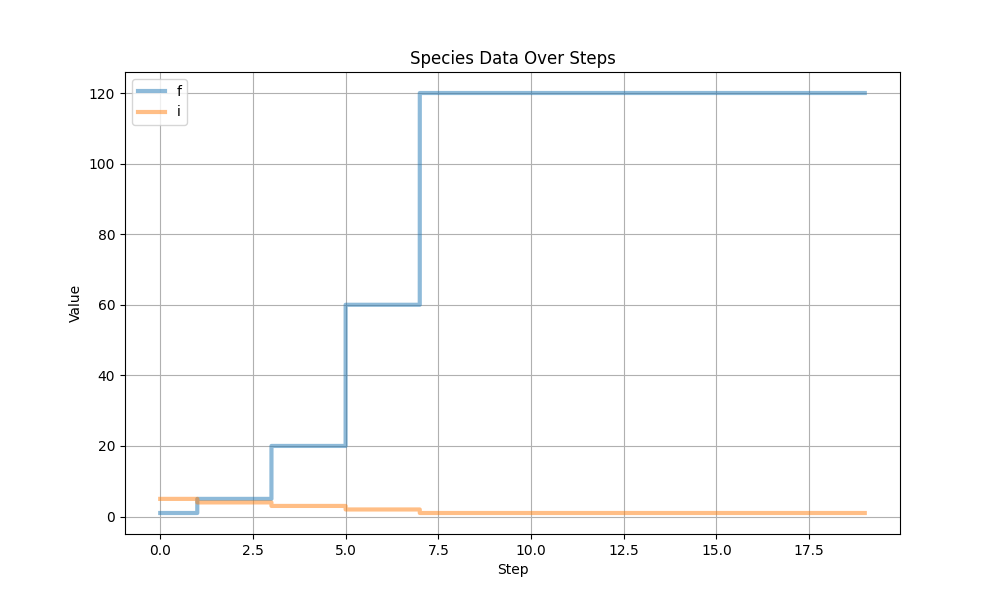
\includegraphics[width=\textwidth]{report/figures/InterpreterPlots/factorialInt.png}
    \caption{Factorial}
\end{figure}

\begin{figure}[H]
    \centering
    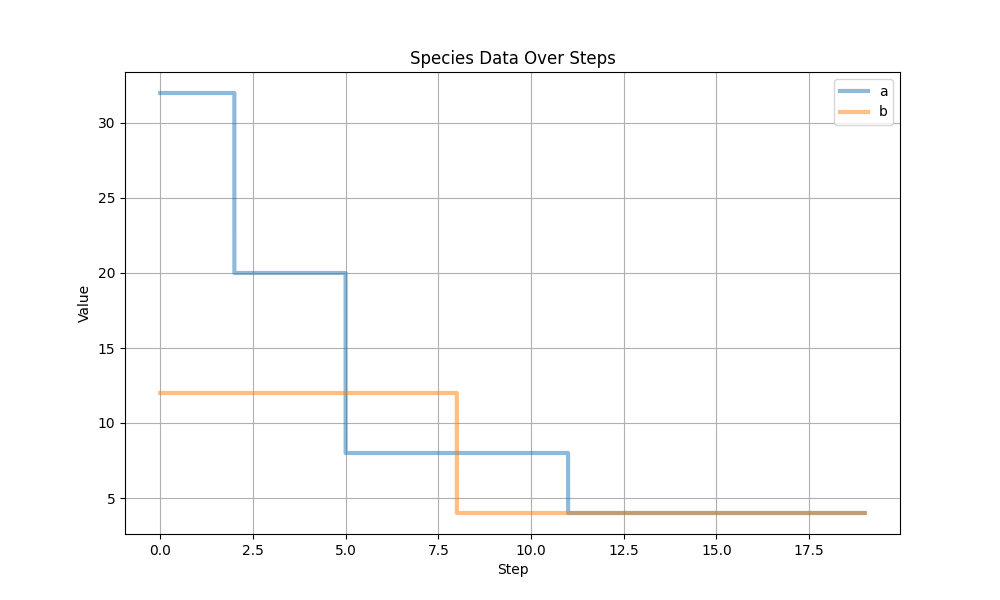
\includegraphics[width=\textwidth]{report/figures/InterpreterPlots/gcdInt.png}
    \caption{GCD}
\end{figure}

\begin{figure}[H]
    \centering
    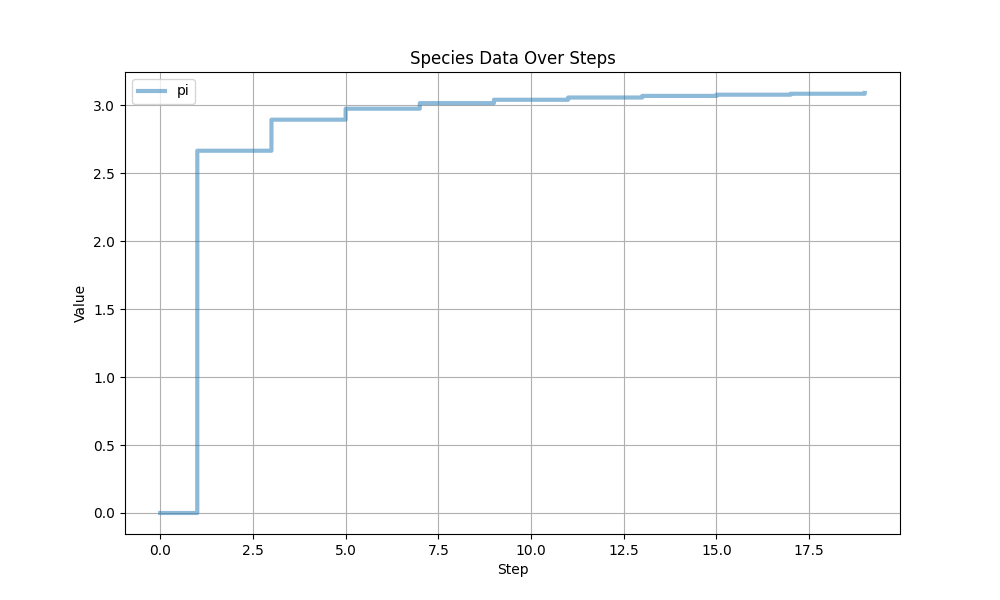
\includegraphics[width=\textwidth]{report/figures/InterpreterPlots/piInt.png}
    \caption{Pi}
\end{figure}

\begin{figure}[H]
    \centering
    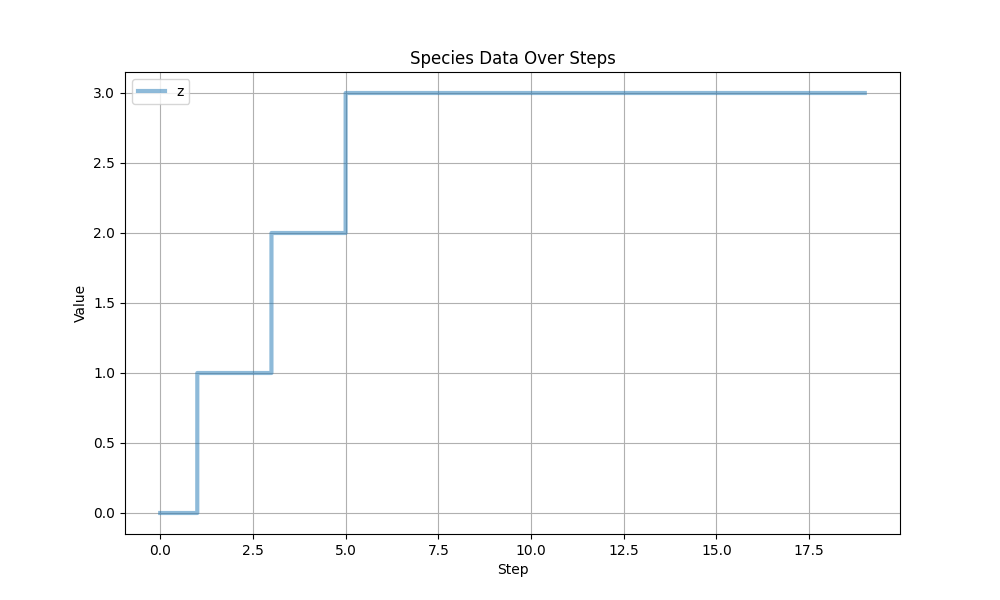
\includegraphics[width=\textwidth]{report/figures/InterpreterPlots/sqrtInt.png}
    \caption{Sqrt}
\end{figure}

\begin{figure}[H]
    \centering
    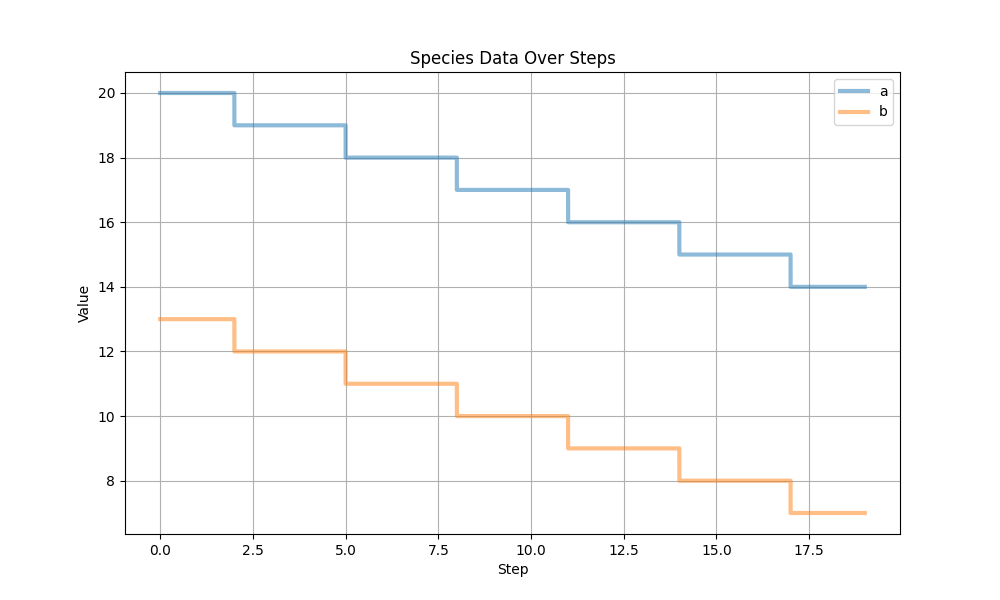
\includegraphics[width=\textwidth]{report/figures/InterpreterPlots/sub2Int.png}
    \caption{Sub2}
\end{figure}




\subsection{Compiler plots}\label{sec:compiler_plots}

\begin{figure}[H]
    \centering
    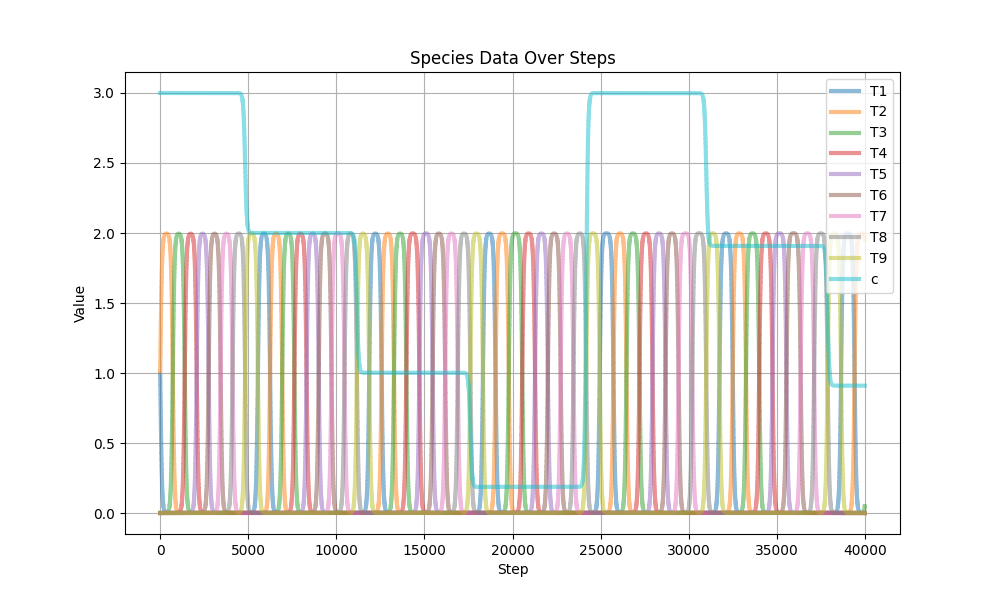
\includegraphics{report/figures/counterWithTimeVars.png}
    \caption{Counter with Time variables}
    \label{fig:counter_time}
\end{figure}

\begin{figure}[H]
    \centering
    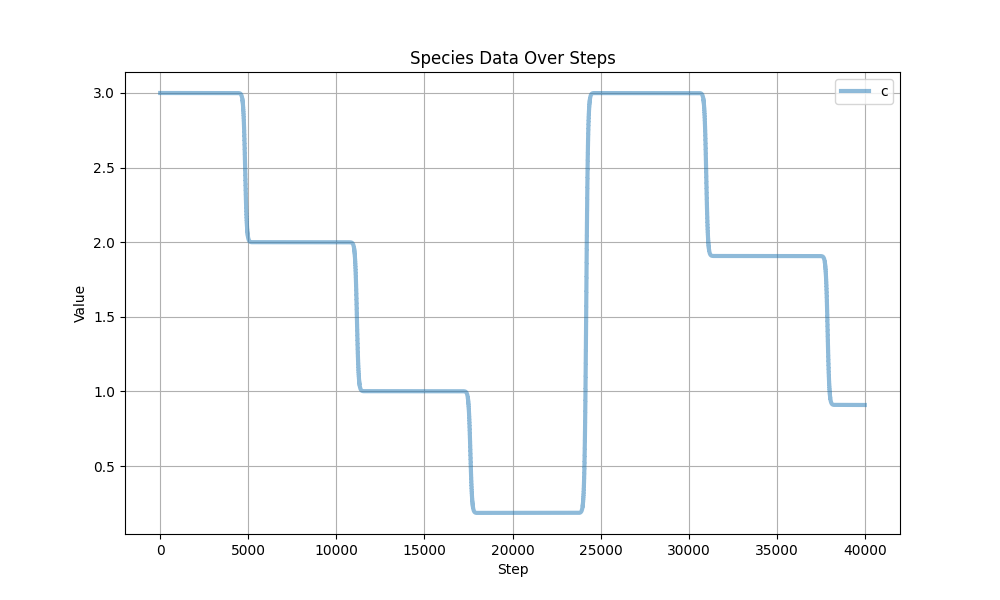
\includegraphics[width=\textwidth]{report/figures/SimulatorPlots/counterSim.png}
    \caption{Counter}
\end{figure}

\begin{figure}[H]
    \centering
    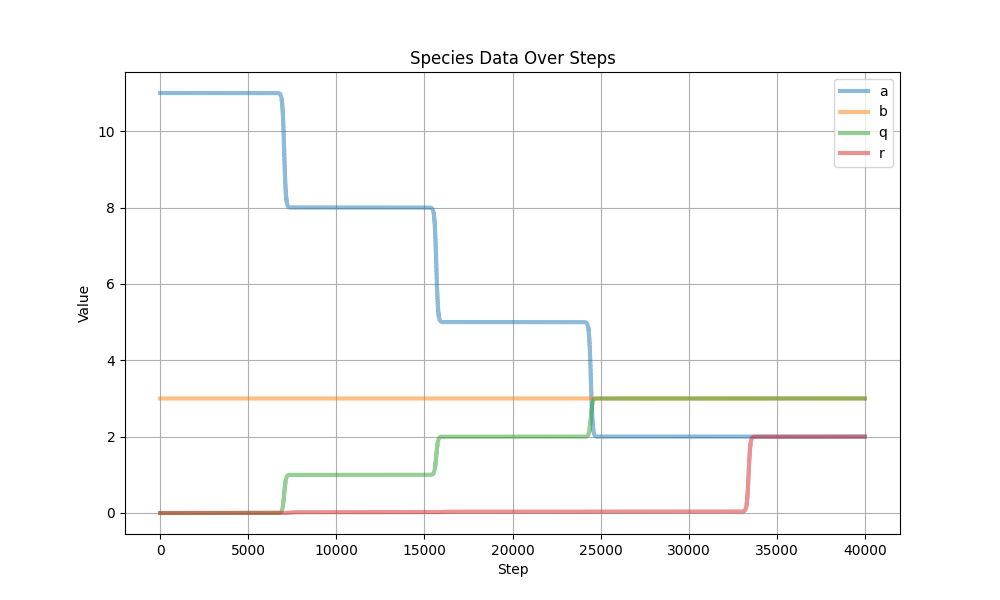
\includegraphics[width=\textwidth]{report/figures/SimulatorPlots/divisionSim.png}
    \caption{Division}
\end{figure}

\begin{figure}[H]
    \centering
    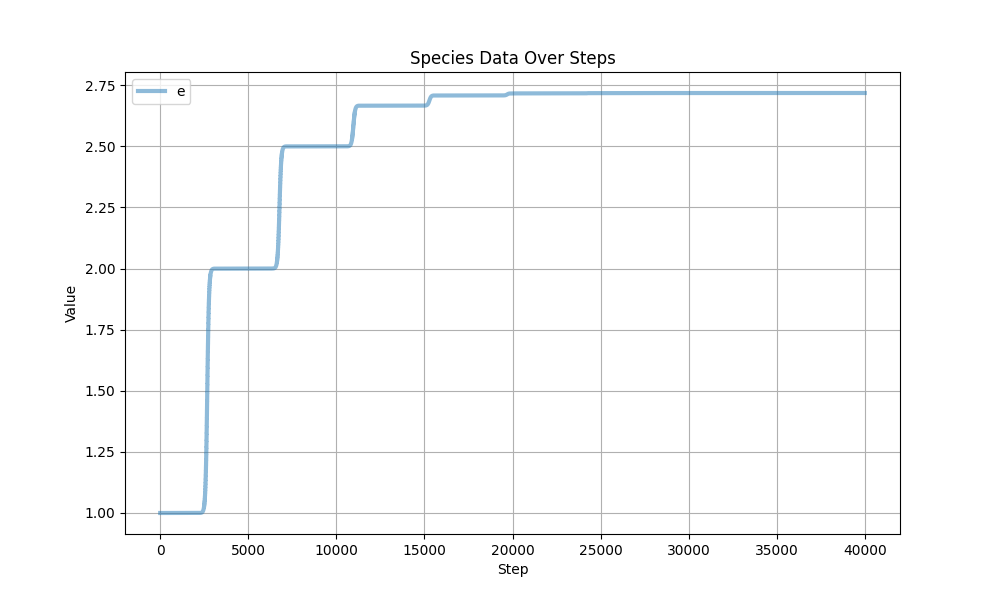
\includegraphics[width=\textwidth]{report/figures/SimulatorPlots/eulerSim.png}
    \caption{Euler}
\end{figure}

\begin{figure}[H]
    \centering
    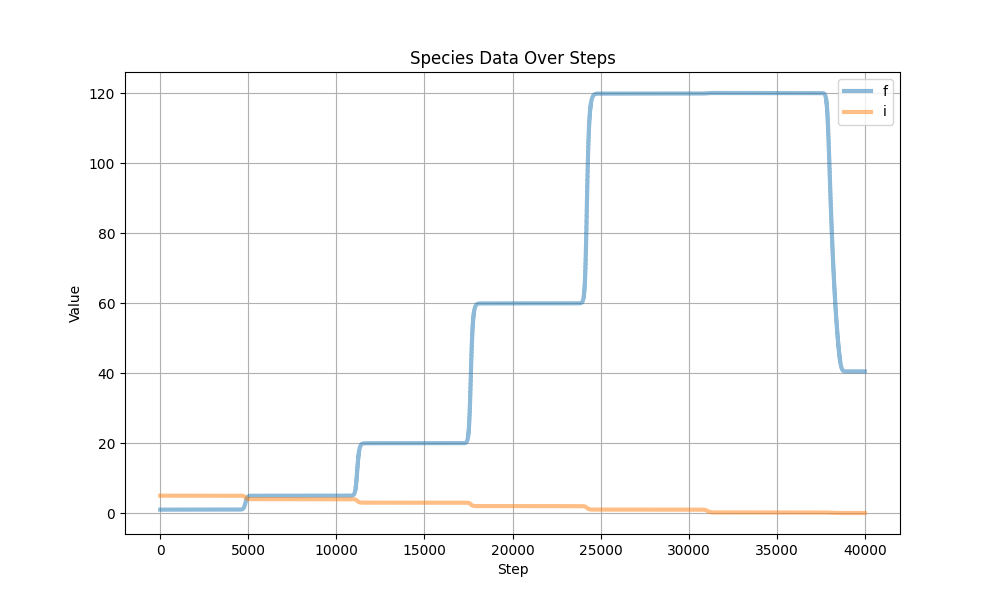
\includegraphics[width=\textwidth]{report/figures/SimulatorPlots/factorialSim.png}
    \caption{Factorial}
\end{figure}

\begin{figure}[H]
    \centering
    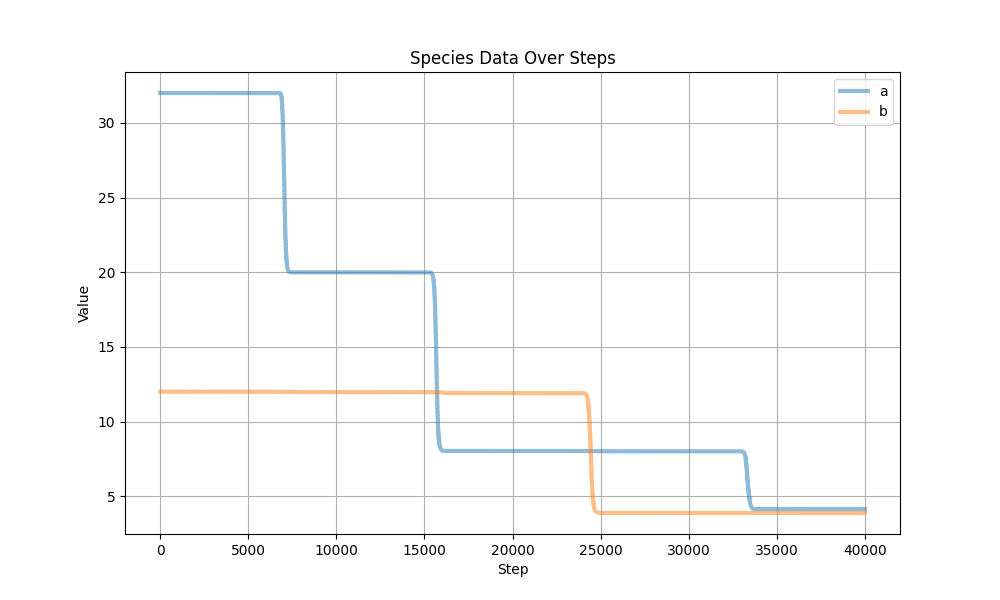
\includegraphics[width=\textwidth]{report/figures/SimulatorPlots/gcdSim.png}
    \caption{GCD}
\end{figure}

\begin{figure}[H]
    \centering
    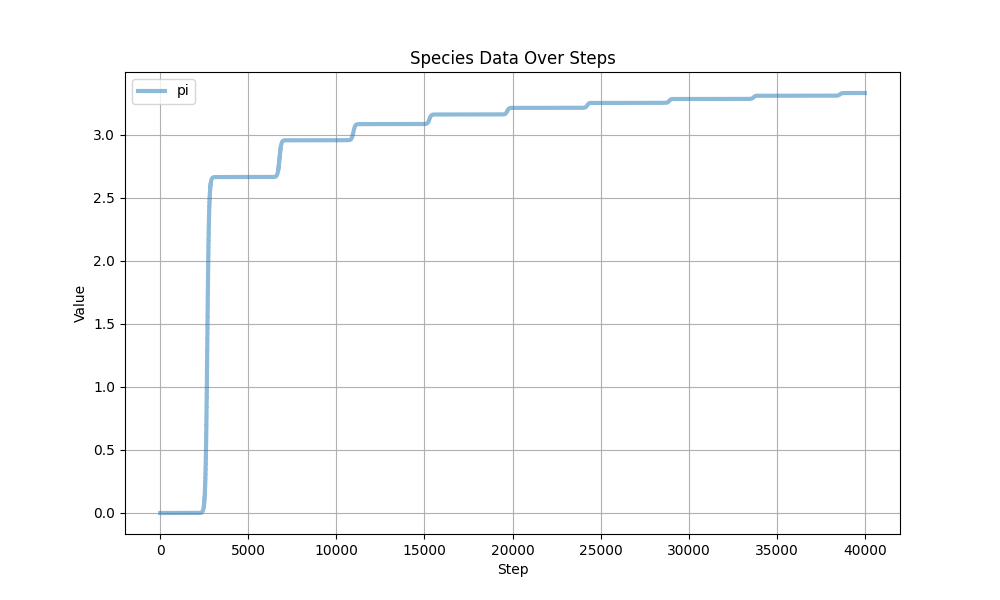
\includegraphics[width=\textwidth]{report/figures/SimulatorPlots/piSim.png}
    \caption{Pi}
\end{figure}

\begin{figure}[H]
    \centering
    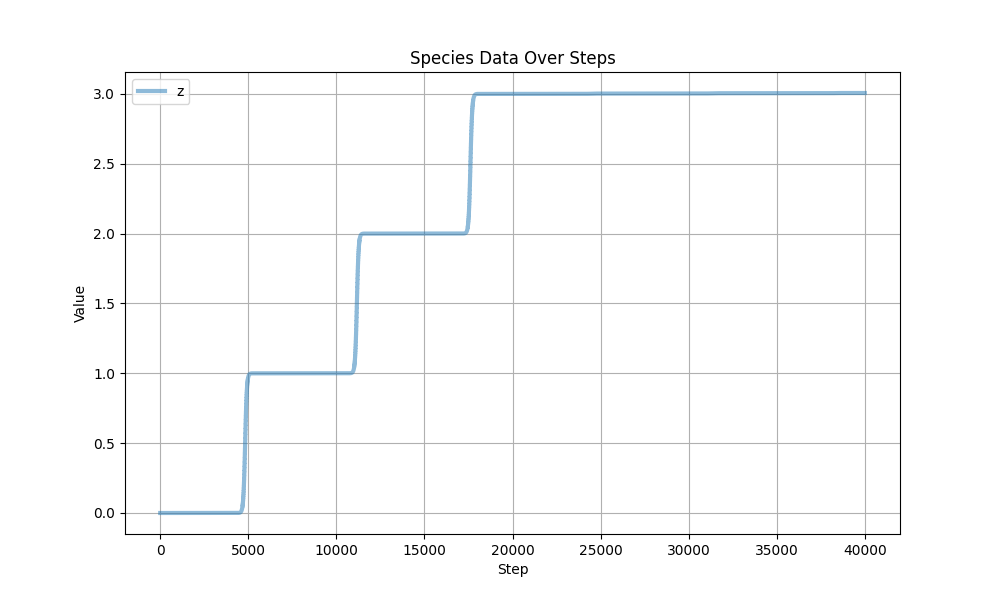
\includegraphics[width=\textwidth]{report/figures/SimulatorPlots/sqrtSim.png}
    \caption{Sqrt}
\end{figure}

\begin{figure}[H]
    \centering
    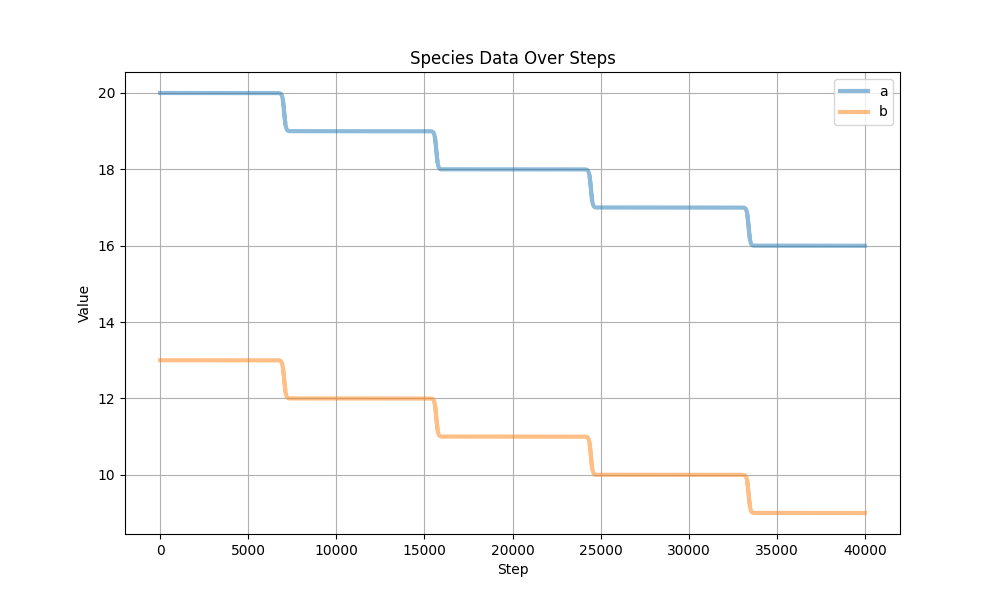
\includegraphics[width=\textwidth]{report/figures/SimulatorPlots/sub2Sim.png}
    \caption{Sub2}
\end{figure}








